\documentclass[10pt,a4paper]{article}
\usepackage[latin1]{inputenc}
\usepackage{amsmath}
\usepackage{amsfonts}
\usepackage{amssymb}
\usepackage{graphicx}
\begin{document}
\section{Descripci�n del problema.}
\section{Herramientas.}
Las herramientas que se pueden usar para abordar la resoluci�n del problema es amplia. Es por ello, que resulta dif�cil elegir la m�s adecuada. Tras un estudio de las bibliotecas disponibles para los distintos lenguajes de programaci�n que domino, me decante por weka(java) y sklearn(python). Tras llevar a cabo la ejecuci�n de distintos algoritmos se obtuvieron los siguientes resultados.
\begin{figure}
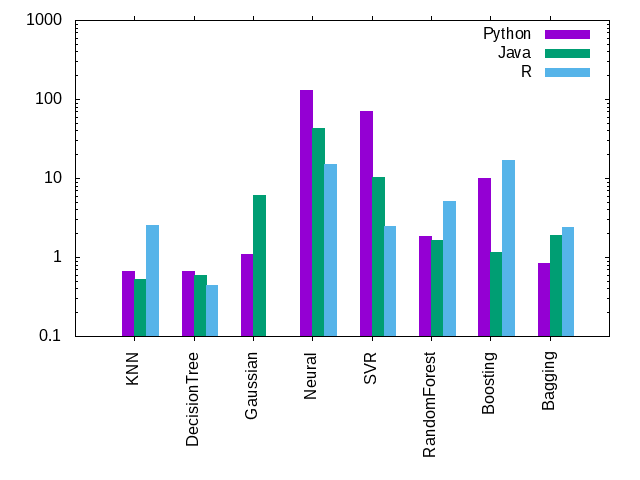
\includegraphics[]{./img/tiempos.png}
\end{figure}
\begin{figure}
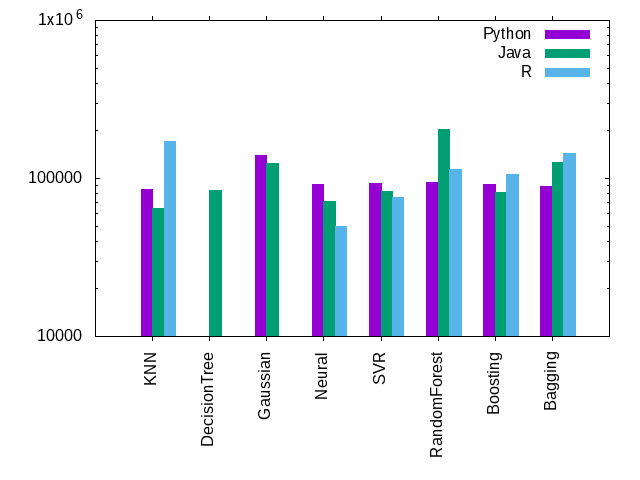
\includegraphics[]{./img/memoria.png}
\end{figure}

Se puede observar que en t�rminos de rendimiento, la librer�a weka es tanto superior a sklearn. Sin embargo, estos dos aspectos no son los �nicos a tener en cuenta.
** weka trabaja con arff
**Es mas facil generar el archivo de resultados en sklearn.
**sklearn mejor documentacion
Estas razones unidas a que la diferencia de rendimiento no es "gran cosa" me hacen decantarme por usar Python. En particular, se usaran las siguientes bibliotecas:
\begin{itemize}
\item NumPy....
\item Pandas...
\item Scikit Learn...
\end{itemize}
\section{Algoritmos.}
\begin{figure}
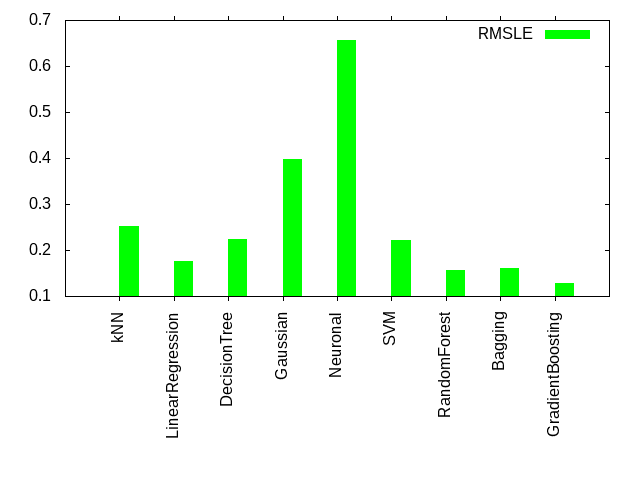
\includegraphics[]{./img/error.png}
\end{figure}
\end{document}